 \begin{center}
	\begin{figure}
		
		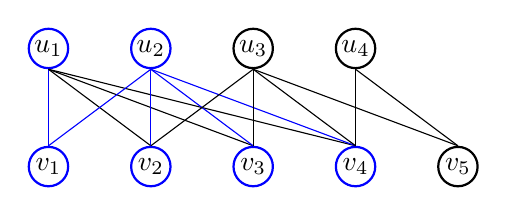
\begin{tikzpicture}[scale=1, every node/.style={circle, draw, minimum size=0.5cm, inner sep=0pt, line width=0.8pt}]
			
			% Nodes
			\node[draw=blue] (u1) at (0,1.5) {$u_1$};
			\node[draw=blue]  (u2) at (1.3,1.5) {$u_2$};
			\node (u3) at (2.6,1.5) {$u_3$};
			\node (u4) at (3.9,1.5) {$u_4$};
			
			\node [draw=blue] (v1) at (0,0) {$v_1$};
			\node [draw=blue] (v2) at (1.3,0) {$v_2$};
			\node [draw=blue] (v3) at (2.6,0) {$v_3$};
			\node [draw=blue] (v4) at (3.9,0) {$v_4$};
			\node (v5) at (5.2,0) {$v_5$};
			% Edges
			\draw [draw=blue] (u1.south) -- (v1.north);
			\draw (u1.south) -- (v2.north);
			\draw (u1.south) -- (v3.north);
			\draw (u1.south) -- (v4.north);
			\draw [draw=blue] (u2.south) -- (v1.north);
			\draw [draw=blue] (u2.south) -- (v2.north);
			\draw [draw=blue] (u2.south) -- (v3.north);
			\draw [draw=blue] (u2.south) -- (v4.north);
			
			\draw (u3.south) -- (v2.north);
			\draw (u3.south) -- (v3.north);
			
			\draw (u3.south) -- (v4.north);
			\draw (u3.south) -- (v5.north);
			
			
			\draw (u4.south) -- (v4.north);
			\draw (u4.south) -- (v5.north);
			
		\end{tikzpicture}
		\caption{An example for $Z_{(2,4)}$}
		\label{fig:z1} 
	\end{figure}
\end{center}


\begin{center}
	\begin{figure}
		
		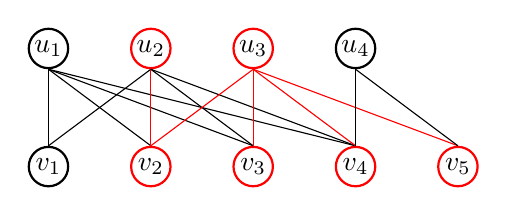
\begin{tikzpicture}[scale=1, 
			every node/.style={circle, draw, minimum size=0.5cm, inner sep=0pt, line width=0.8pt}
			]
			
			% Nodes
			\node (u1) at (0,1.5) {$u_1$};
			\node[draw=red] (u2) at (1.3,1.5) {$u_2$};
			\node [draw=red](u3) at (2.6,1.5) {$u_3$};
			\node (u4) at (3.9,1.5) {$u_4$};
			
			
			\node (v1) at (0,0) {$v_1$};
			\node[draw=red] (v2) at (1.3,0) {$v_2$};
			\node[draw=red] (v3) at (2.6,0) {$v_3$};
			\node [draw=red](v4) at (3.9,0) {$v_4$};
			\node [draw=red](v5) at (5.2,0) {$v_5$};
			
			% Edges
			\draw (u1.south) -- (v1.north);
			\draw (u1.south) -- (v2.north);
			\draw (u1.south) -- (v3.north);
			\draw (u1.south) -- (v4.north);
			\draw (u2.south) -- (v1.north);
			\draw[draw=red] (u2.south) -- (v2.north);
			\draw (u2.south) -- (v3.north);
			\draw (u2.south) -- (v4.north);
			
			\draw [draw=red](u3.south) -- (v2.north);
			\draw [draw=red](u3.south) -- (v3.north);
			
			\draw [draw=red](u3.south) -- (v4.north);
			\draw [draw=red](u3.south) -- (v5.north);
			
			
			\draw (u4.south) -- (v4.north);
			\draw (u4.south) -- (v5.north);
			
		\end{tikzpicture}
		\caption{Another for $Z_{(2,4)}$}
		\label{fig:z2} 
	\end{figure}
\end{center}